\documentclass[11pt,a4paper]{article}
\usepackage[utf8]{inputenc}
\usepackage[T1]{fontenc}
\usepackage{textgreek}
\usepackage{amsmath}
\usepackage{booktabs}
\usepackage{hyperref}
\usepackage{multicol}
\usepackage{graphicx}
\usepackage[margin=2cm]{geometry}

\setlength{\columnsep}{1cm}

\title{\vspace{-0.5cm}\textit{SnapBind}: Lightweight CNN for Protein Binding Pocket Prediction}
\author{David Z Barth, Alexander Haas, Elias M Bruss}
\date{}

\begin{document}

\vspace{1cm}
\maketitle
\vspace{-0.3cm}

\begin{multicols}{2}

\section*{Abstract:} We present \textit{SnapBind}, a lightweight CNN (0.5M parameters) for predicting protein druggability and binding pockets from amino acid sequences. Using 100k protein-ligand pairs from BindingDB, our model enables local deployment for high-throughput screening without expensive computational infrastructure.

\section{Methods}

\noindent \quad \textbf{Dataset:} 100k protein-ligand pairs from BindingDB plus 20k negative controls (Antibodies, structural proteins, nucleases). Binding sites defined by 5Å cutoff with binary residue annotation. \\

\noindent \quad \textbf{Architecture:} FastCNNBindingPredictor with 64-dim embeddings, 128-dim hidden layers, 0.1 dropout, handling 20-300 residue sequences.\\

\noindent \quad \textbf{Training:} Batch size 32, AdamW (lr=2e-4), focal loss (α=1, γ=2) for class imbalance, early stopping, Apple Silicon GPU acceleration.

\section{Progressive Design}

Three-pass architecture: (1) Sequence-based CNN for druggability, (2) ESM embeddings for evolutionary context, (3) SMILES integration for small-molecule ligand-specific predictions.

\section{Results}

\textbf{Efficiency:} 0.5M parameters enable consumer hardware deployment with rapid batch processing and local execution. \\

\textbf{Performance:} Stable training with effective class imbalance handling through focal loss and positive class weighting.

\begin{center}
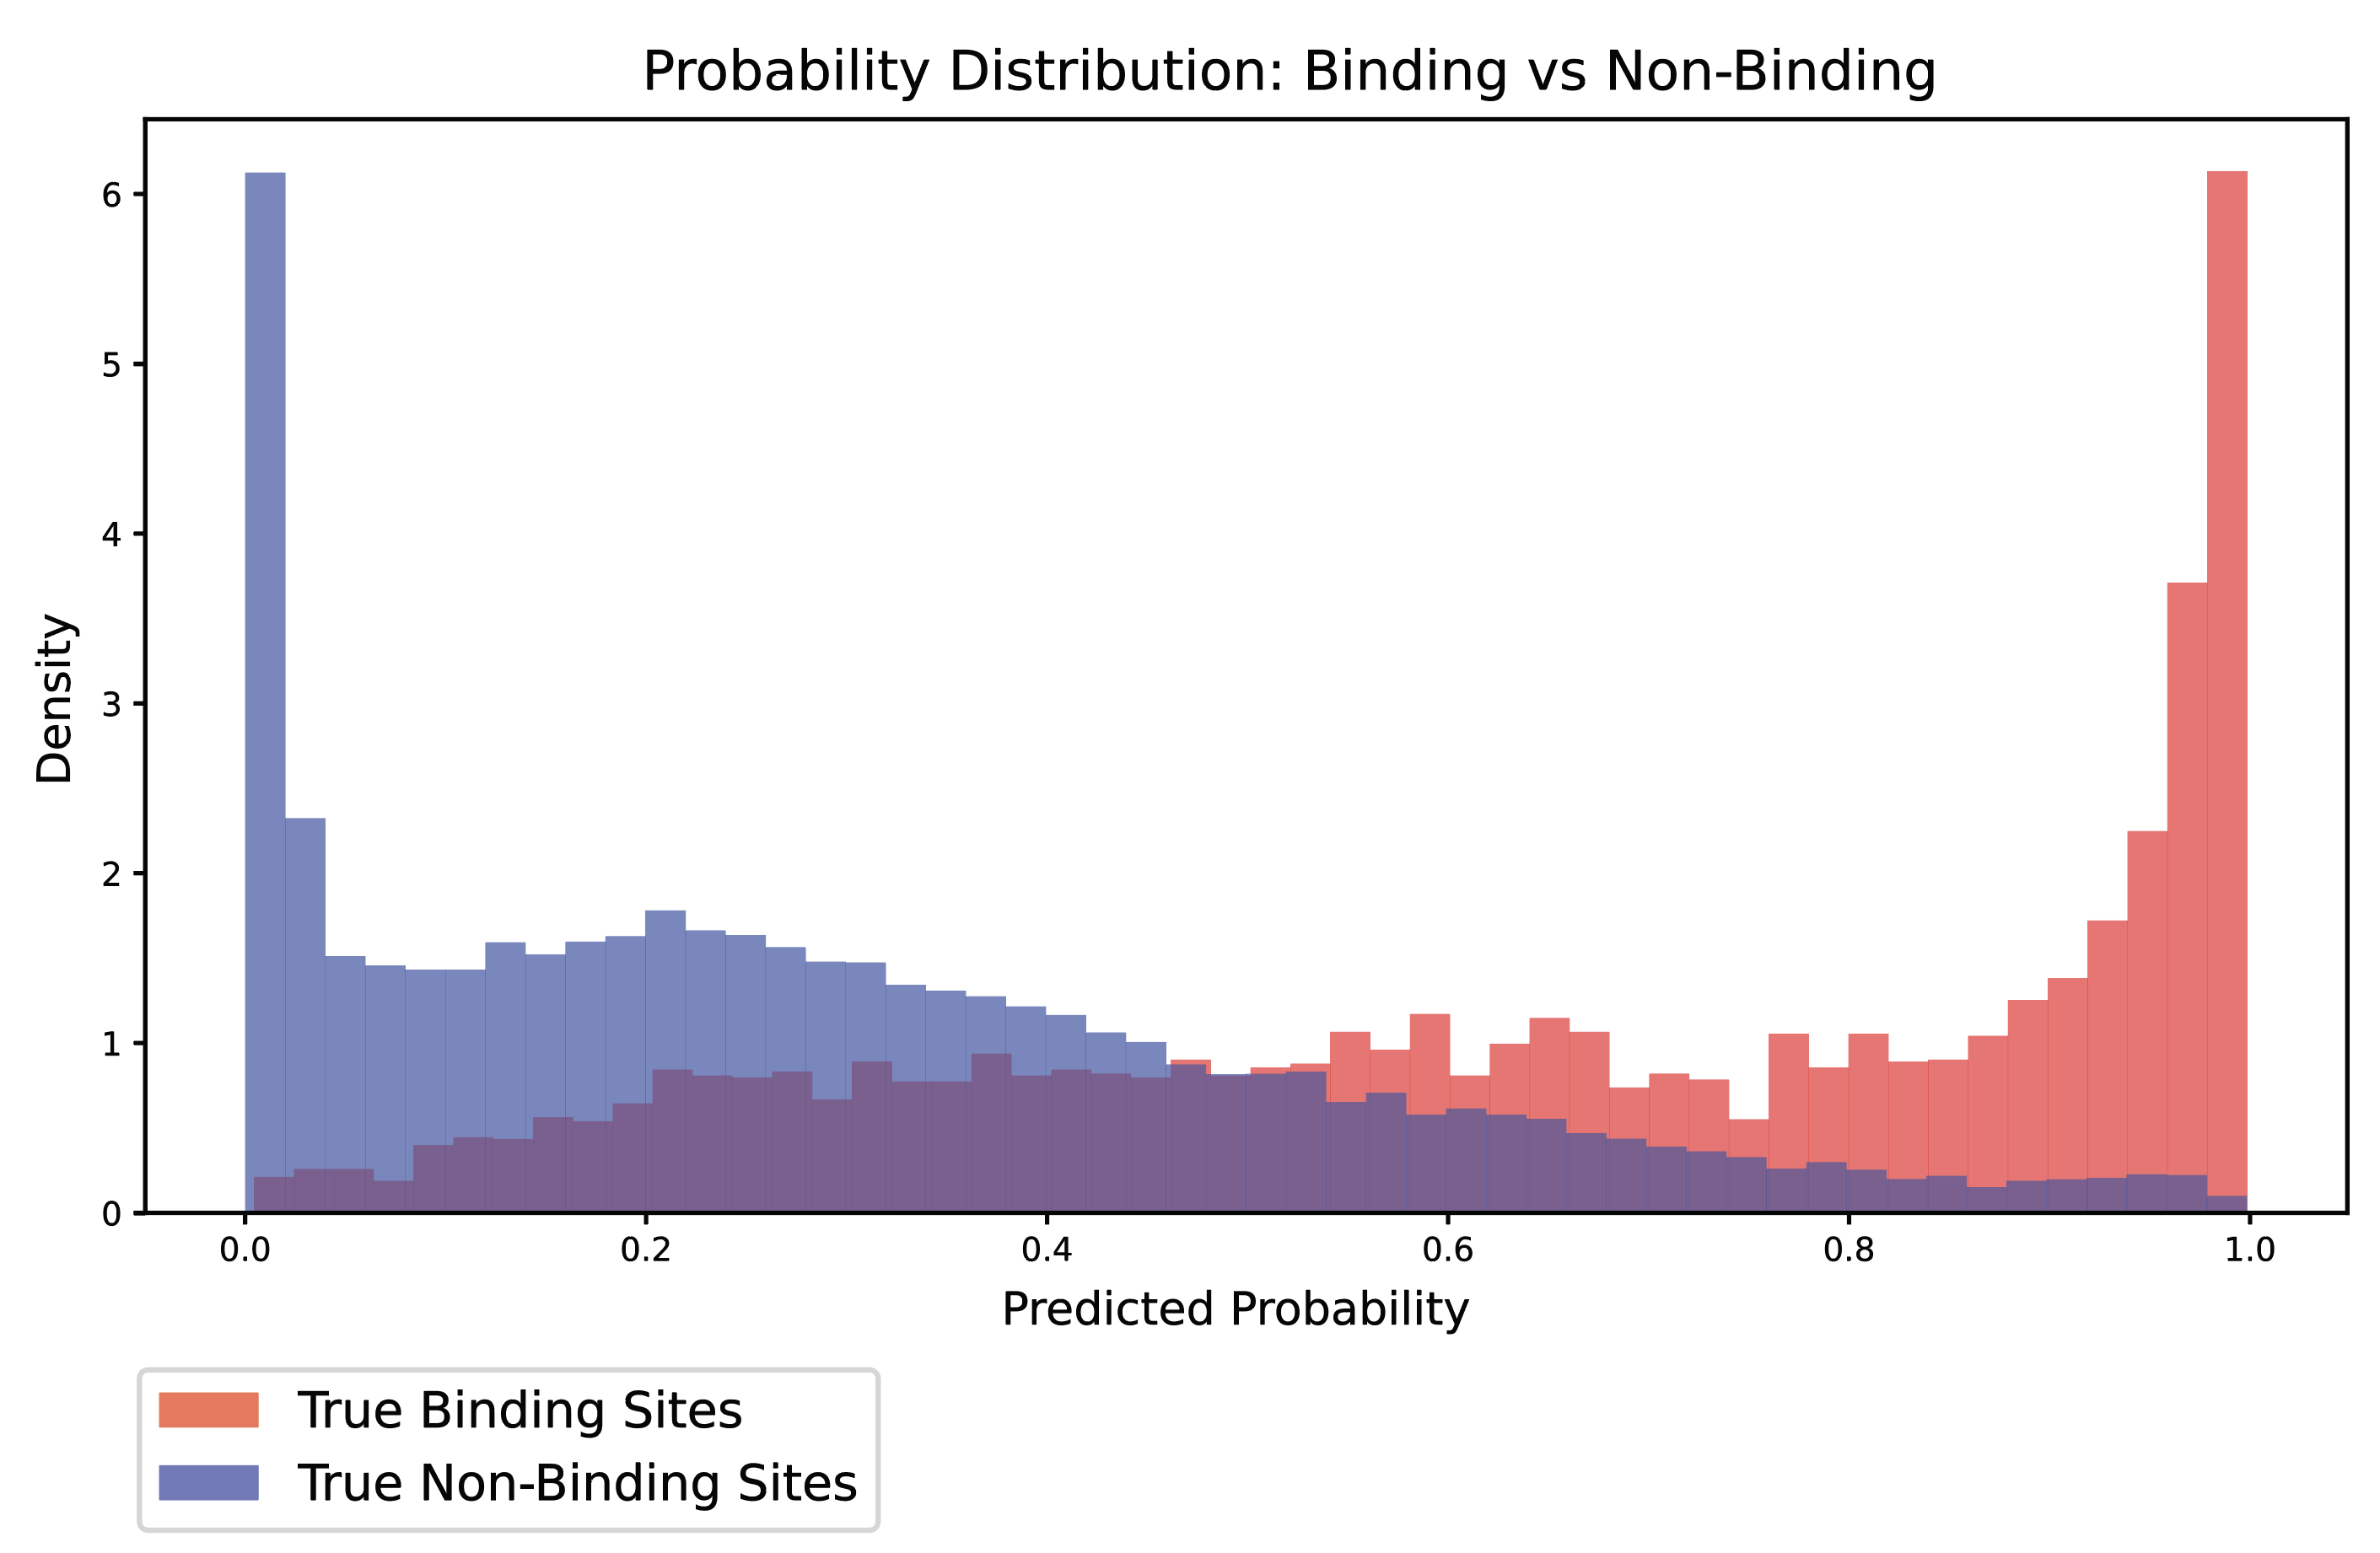
\includegraphics[width=1\columnwidth]{fig1mod.png}
\\[0.1cm]
\textbf{Figure 1:} Score distribution for ground truth.
\end{center}

\section{Applications}

High-throughput protein screening, binding site localization, academic accessibility without proprietary platforms, local computational pipeline integration.

\section{Conclusion}

Our lightweight CNN democratizes binding pocket prediction by balancing performance with computational efficiency, enabling researchers to perform drug discovery screening without extensive infrastructure requirements.

\end{multicols}

\vfill

\end{document}